\documentclass[border=10pt]{standalone}
\usepackage{pgfplots}
\usepgfplotslibrary{colormaps}
\pgfplotsset{trig format plots=rad}
\begin{document}
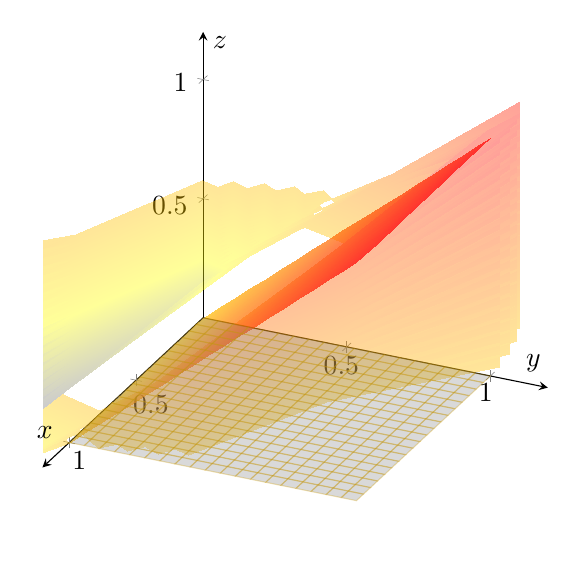
\begin{tikzpicture}
\begin{axis}[
    width=8cm, height=8cm,
    view={115}{30},
    xlabel=$x$, ylabel=$y$, zlabel=$z$,
    xmin=0, xmax=1.2, ymin=0, ymax=1.2, zmin=0, zmax=1.2,
    axis lines=center,
    grid=major
]
% The cylinder surface x^2 + y^2 = 1 in the first octant
% x = cos(theta), y = sin(theta), z in [0, sin(theta)]
\addplot3[surf, domain=0:pi/2, y domain=0:1, samples=20, opacity=0.4, color=blue, shader=interp] 
    ({cos(deg(x))}, {sin(deg(x))}, {y*sin(deg(x))});

% The plane z = y over the region x^2 + y^2 <= 1, x >= 0, y >= 0
\addplot3[surf, domain=0:1, y domain=0:1, samples=20, opacity=0.5, color=red, shader=interp] 
    ({x}, {y}, {y});
% This might not be correctly bounded. 
% Let's use a safer approach for the plane z = y over the quarter disk.
% We can use the domain where x^2 + y^2 <= 1.
\addplot3[surf, domain=0:1, y domain=0:1, samples=20, opacity=0.4, color=red, shader=interp]
    ({x}, {y}, {y});
% Actually, just plotting the surface z=y and clipping it or using polar is better.
% But for a simple visualization:
\addplot3[surf, domain=0:1, y domain=0:1, samples=20, opacity=0.3, color=gray] 
    ({x}, {y}, {0}); % base z=0

\end{axis}
\end{tikzpicture}
\end{document}
